\chapter{Inputting the system into the IDF file}\label{inputting-the-system-into-the-idf-file}

Since, it is not possible to input schematics into the input file, it is important to add descriptive comments to all of the entries to ensure that all the components in the system have been accounted for. Such documentation will also make debugging easier. It should be noted that all of the syntax for the inputs is documented in the Input-Output reference guide. A flowchart for the basic input process is provided in Figure~\ref{fig:flowchart-for-input-process}.

\begin{figure}[hbtp] % fig 11
\centering
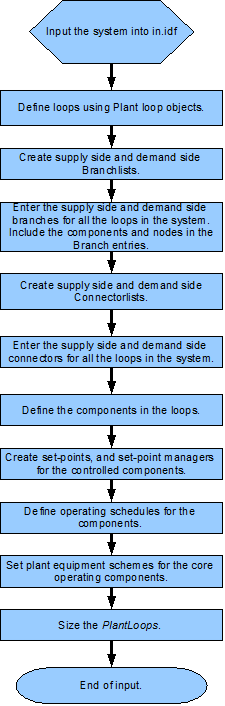
\includegraphics[width=0.9\textwidth, height=0.9\textheight, keepaspectratio=true]{media/image011.png}
\caption{Flowchart for input process \protect \label{fig:flowchart-for-input-process}}
\end{figure}
